\documentclass[12pt]{article}
\usepackage[utf8]{inputenc}
\usepackage[slovene]{babel}

\usepackage{hyperref}
\usepackage{listings} % za naslovnico
\usepackage{amsthm}
\usepackage{amsmath, amssymb, amsfonts}
\usepackage{graphicx}


%\graphicspath{ {./Slike/} }
\usepackage{subcaption} % za side-by-side slike
\usepackage[]{algorithm2e}
\usepackage[
top    = 1.5cm,
bottom = 2.cm,
left   = 2.cm,
right  = 2.cm]{geometry}

\usepackage{footnote}
\usepackage{hyperref}
\hypersetup{
    colorlinks=true,
    linkcolor=blue,
    filecolor=magenta,      
    urlcolor=cyan
    }

\makesavenoteenv{tabular}
\title{Domača naloga - 2.del \\
\large Verjetnostne gramatike in posodabljanje verjetnosti}

\begin{document}
    
\author{Vito Rozman}
\date{\today}
\maketitle

\section{Psevdo koda algoritma}

Spodaj je psevdo koda algoritma za verjetnostne gramatike. Najprej je potrebno ustavriti 
objekt \textbf{eqAlgo}, ki spejme levo in desno stran spemenljivk v enačbi, gramatiko, 
podatke in število generiranja enačb ob vsaki iteraciji. Potem za zagon 
algoritma definitamo objektno funkcijo \textbf{model},
kjer podamo število iteracij ($Iter$), željeno napako ($loss$) in 
parameter posodabljanja verjetnosti ($\Delta$).\\


\begin{algorithm}[H]
    \KwData{$Iter$, $loss$, $\Delta$}
    \KwResult{Napaka enačbe, Dobljena enačba}
    
    \For{$i = 0, \dots, Iter$}{
        ($\text{NAPAKA}_i$, $\text{ENAČBA}_i$) = \textbf{GenerirajEnačbo()}\\        
        \If{$\text{NAPAKA}_i$ $<$ $loss$}
            {Vrni: $\text{NAPAKA}_i$, $\text{ENAČBA}_i$}
        \ElseIf{$\text{NAPAKA}_i$ $<$ $\text{NAPAKA}_{i-1}$}
            {\textbf{PosodobiVerjetnosti}($\text{ENAČBA}_i$, $\Delta$)}
        \ElseIf{$\text{NAPAKA}_i$ $\geq $ $\text{NAPAKA}_{i-1}$}
            {\textbf{PosodobiVerjetnosti}($\text{ENAČBA}_{i-1}$, $\Delta$)}
        \ElseIf{$(\text{NAPAKA}_i - \text{NAPAKA}_0$ $\geq$ $\text{NAPAKA}_0 - \text{BestNAPAKA})$ or 
        $(i \in [20, 40, 60, ...])$}
        {\textbf{PosodobiVerjetnosti}($\text{BestENAČBA}$, $\Delta$)}
        Zapomni si vse porebne spremenljivke za naslednje korake
    }
    \textbf{Vrni:} $\text{BestNAPAKA}$, $\text{BestENAČBA}$\\
\end{algorithm}

\section{Rezultati}

Na sliki \ref*{rezultati} so rezutati primerjave razvitega verjetnostnega algoritma in 
algoritma, ki vzorči enačbe nalključno. Pri enačbi 
\ref*{fig:subim2} se je algoritem najbolje izkazal, ker je enačbo našel že v $400$ iteracijah. 
Pri enačbi \ref*{fig:subim1} se model ni tako dobro iskazal, kar bi morda lahko pomenilo 
da gramatika ni tako dobra za dano enačbo. V primeru \ref*{fig:subim3} pa vidimo 
da bi algoritem morda našel enačbo z višanjem iteracij.
\begin{figure}[h!] % <---
    \begin{subfigure}{0.32\textwidth}
        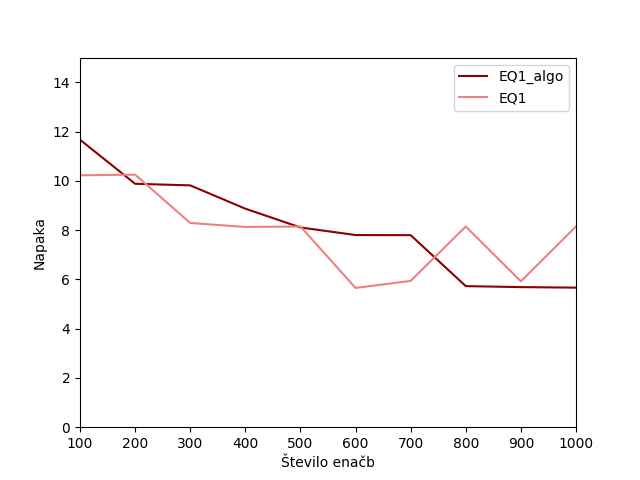
\includegraphics[width=\linewidth,  height=4.4cm]{Fig/eq1.png}
        \caption{$y = x_1 - 3x_2 - x_3 - x_5$}
        \label{fig:subim1}
    \end{subfigure}
 \hfill % <--- 
    \begin{subfigure}{0.32\textwidth}
        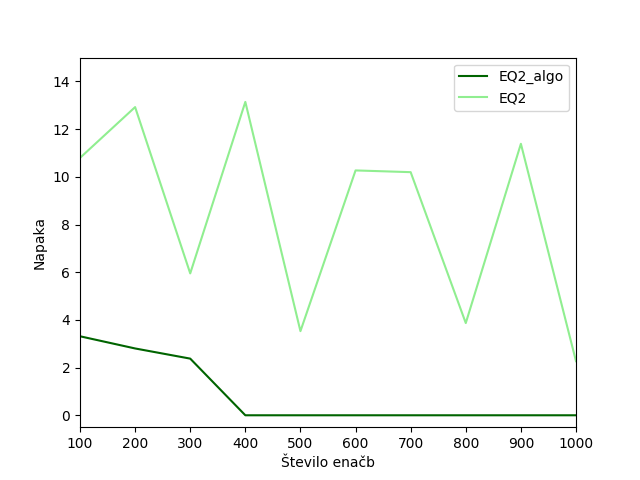
\includegraphics[width=\linewidth,  height=4.4cm]{Fig/eq2.png}
        \caption{$y = x_1^5x_2^3$}
        \label{fig:subim2}
    \end{subfigure}
 \hfill % <---
    \begin{subfigure}{0.32\textwidth}
        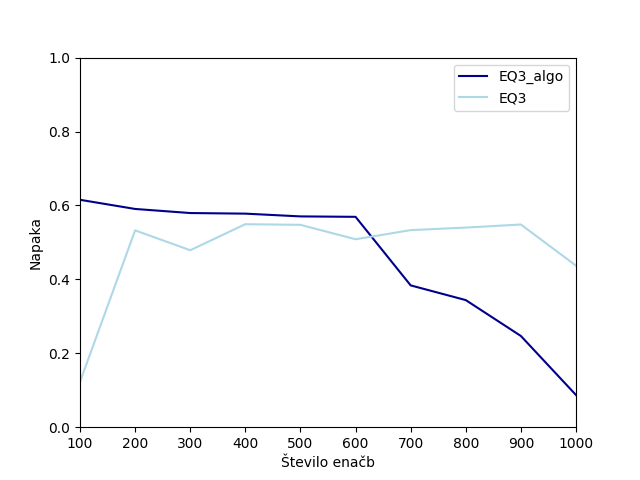
\includegraphics[width=\linewidth,  height=4.4cm]{Fig/eq3.png}
        \caption{$y = \sin(x_1) + \sin(\frac{x_2}{x_1^2})$}
        \label{fig:subim3}
    \end{subfigure}
 
    \caption{Primerjave delovanja verjetnostnega algoritma}
    \label{rezultati}
 \end{figure}



\section{Komentarji in možne izboljšave}
Algoritem sem napisal tako da lahko sprejme poljubno gramatiko. V ta namen sem uvedel nov 
objekt v obliki slovarja 
\{spremenljivka : \{pravilo : verjetnost pravila, \dots
    \},\dots
\}, ki mi je omogočil dokaj hitro posodabljanje verjetnosti.
Za posodabljanje verjetnosti sem testiral dva pristopa softmax in fullfill s predpisoma:
\begin{align*}
   \text{Softmax: } p_i = \frac{\exp^{p_i \pm \Delta}}{\sum_{j}{\exp^{p_j \pm \Delta}}}, \quad
   \text{Fulfill: } p_i = \frac{(p_i \pm \Delta)_{+}}{\sum_{j}{(p_j \pm \Delta)_{+}}}.
\end{align*}
Softmax se ni iskazal za dobro ker so vhodne verjetnosti med $0$ in $1$, in  bi moral 
paramater 
$\Delta$ izbirati bolj pametno, zato sem raje uporabljal fulfill. Paziti sem moral tudi 
na robne primere, ker če ima gramatika rekurzivna pravila, morajo vseeno obstajati pravila 
ki niso rekurzivna s pozitivno verjetnostjo, ker drugače se model zacikla.

Ob testeranju sem ugotovil da model ne deluje presenetljivo hitreje od naključnega vzorčenja, 
kar je morda posledica večanja števila enačb ob robnih izidih (vidno v kodi). Druga izpopolnitev
bi bila lahko, da glede na dano napako posodablja verjetnosti in ne s fiksnim korakom $\Delta$.
Kot zadnje, če se napaka modela oddaljuje od začetne napake (in tudi vakih 10 iteracij), 
postavim model v njegovo najboljše stanje do tega trenutka,
v tem primeru bi lahko drugače posodobil verjetnosti (morda za manjšo vrednost).


\section*{Dodatni napotki ob zagonu algoritma}
Algoritem poženemo kot je opisenao zgoraj. V skripti \textbf{algo.py} se nahaja rared 
z implementacijo algoritma. Na dnu kode je zakomentiran primer enega zagona algoritma.
Uporabljena knjižnjica je \textbf{ProGED} (verzija $0.8.5$), ki jo v času razvijanja 
algoritma nisem posodobil!


\end{document}